%!TEX root = ../template.tex
%%%%%%%%%%%%%%%%%%%%%%%%%%%%%%%%%%%%%%%%%%%%%%%%%%%%%%%%%%%%%%%%%%%%
%% chapter2.tex
%% NOVA thesis document file
%%
%% Chapter with the template manual
%%%%%%%%%%%%%%%%%%%%%%%%%%%%%%%%%%%%%%%%%%%%%%%%%%%%%%%%%%%%%%%%%%%%

\typeout{NT FILE chapter2.tex}%

% Define the definition environment
\newenvironment{definition}[1][Definition]{%
    \par\vspace{10pt}\noindent\textbf{#1.}
}{%
    \par\vspace{0pt}
}

\chapter{Background}
\label{cha:background}

This chapter will introduce the foundational knowledge necessary to understand
runtime verification. We will start by defining classical terminology,
including specification languages and monitors. We will clarify what it means
for a process to be monitorable, followed by discussing various deployment and
instrumentation techniques that can be utilized. Additionally, we will explore
how the actor-based model can be leveraged within runtime verification and why
it is a good abstraction for runtime verification.

\section{Runtime Verification}
\label{sec:runtime_verification}
Runtime verification (RV) is a field in formal methods that deals with the study,
orchestration,  and application of techniques that grant one the ability to
verify if a given run of a system under scrutiny (SUS) satisfies or violates a
given behaviour~\cite{leucker2009brief}.

RV operates on the execution trace of a running system, verifying formal
properties with the traces of events incrementally generated by the system;
this makes it distinguishable from other approaches~\cite{falcone2012can}.

The essence of RV lies in generating a monitor from a
high-level specification language that outlines the properties to be monitored
during runtime; essentially, the properties that the SUS must adhere
to~\cite{bartocci2018introduction}. This process automatically synthesises a
monitor based on a correctness property, denoted as $\phi$, described in a
specification language. The generated monitor is then employed to observe
either the ongoing execution of the system or a recorded history of its
execution to check whether it adheres to property $\phi$.

In more formal terms, if $\mathcal{L}(\phi)$ represents the set of valid
executions defined by the property $\phi$, then runtime verification can be
boiled down to verifying whether the current execution, denoted as $w$, is part
of that set, $w \in \mathcal{L}(\phi)$~\cite{bauer2011runtime}; this is known as the word problem.

Runtime verification revolves around three core questions: how to formally
define desired and undesired behaviours, how to synthesise executable monitors
from high-level specifications, and how to instrument these monitors with the
system under scrutiny efficiently. Addressing these questions is
essential for building any effective RV framework.

\subsection{Terminology}
\label{sub_sec:terminology}
In RV, terminology is often used broadly, and definitions can vary
significantly depending on the context. The terminology for concepts like
monitorability varies widely, with differing interpretations despite attempts
at standardization~\cite{bartocci2018introduction,leucker2009brief,
teachingRV, ferrando2025towards}. To ensure clarity and
simplicity in this part of the document, we will introduce some basic notions
of RV in straightforward terms, as presented in~\cite{falcone2021taxonomy}. A more
detailed discussion and precise definitions will follow in subsequent sections,
depending on the level of detail needed in those contexts. In
\Cref{fig:instrumenation} (adapted from~\cite{bartocci2018introduction}), we
can see an overview of these concepts and the main structure of RV frameworks.

\begin{figure}[htbp]
  \centering
  \includegraphics[width=0.75\linewidth]{Chapters/Figures/newOnlineMonitor.pdf}%
  \caption{A basic RV setup}
  \label{fig:instrumenation}
\end{figure}
An event refers to a produced action of a system that can be observed. A trace
is a sequence of events generated by the system. A trace is an abstraction of a
single system run, represented as a finite sequence of events. Although
a system could run indefinitely and produce an infinite trace, RV works with
finite traces. Therefore, a trace in this context will be a prefix of the
infinite trace the system is producing.

A property is intuitively something that one expects the SUS to adhere to.
These properties can be formally defined using a specification language, which
provides a concrete property description. More rigorously, a property can be
seen as a set of traces, representing a partition of the set of all possible
traces of the system, as described by Falcone et
al.~\cite{falcone2021taxonomy}. A specification explicitly describes a
property that is defined using a specification language. This language defines
the expected behaviour of the system. A specification language is a formalism
that describes a property, such as regular expressions or automata, each
providing a different approach to specifying the same underlying behaviour.

A monitor is a runtime entity automatically derived from a formal property
specification. Executing in parallel with the system, it observes relevant
events and determines whether the property is satisfied or violated during
execution. It reads the system's trace incrementally and produces a verdict,
alerting the SUS or, in some cases, even steering it when a property violation
occurs. A verdict is the monitor's result, usually expressed as a value from a
given truth domain. The simplest form of a verdict is a binary value, such as
true or false. However, as explored further in the document, truth domains may
allow for additional verdict values beyond these two.

Instrumentation is the computational link connecting the system's execution
with the monitor's analysis. It involves extracting traces from the system and
feeding them into the monitor. It also addresses how the system and monitor are
deployed and run in parallel~\cite{bartocci2018introduction}.

\newtheorem{thm}{Theorem}[section]
\newtheorem{example}{Example}

\begin{example}
\normalfont
This chapter introduces a simple chat room system as the running example. The
  system can be instrumented to capture both the events it produces and the
  messages exchanged within the chat. These events need not be limited to
  primitive actions but may also carry contextual information, such as the
  specific chat room in which a user posts a message. On this basis, we can
  define several correctness properties to govern the system’s behaviour. For
  instance, a user must \texttt{login} before entering a chat room; once
  inside, the user may \texttt{post} messages; and before logging out, the user
  must first \texttt{leave} the room. Taken together, these rules characterise
  the intended session behaviour of the system. Such behaviour can be formally
  expressed in a specification language, for example, through automata, as
  illustrated in \Cref{fig:running_examplee}.
\label{test example}
\end{example}

\begin{figure}[htbp]
\centering
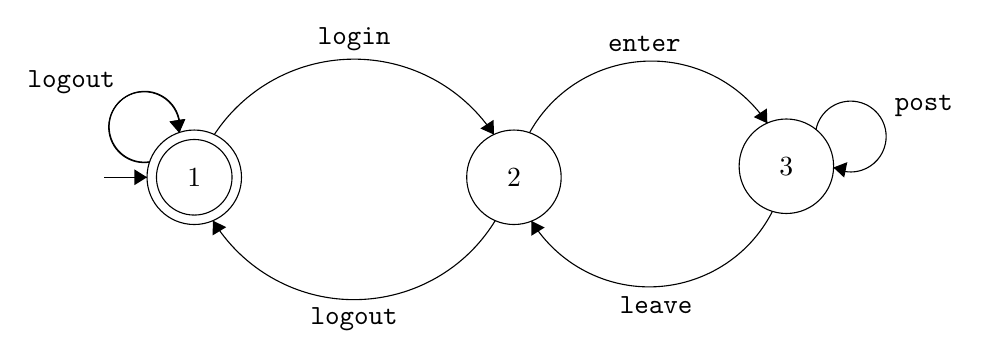
\begin{tikzpicture}[scale=0.2]
\tikzstyle{every node}+=[inner sep=0pt]
\draw [black] (17.7,-29.8) circle (3);
\draw (17.7,-29.8) node {$1$};
\draw [black] (17.7,-29.8) circle (2.4);
\draw [black] (38,-29.8) circle (3);
\draw (38,-29.8) node {$2$};
\draw [black] (55.3,-29.1) circle (3);
\draw (55.3,-29.1) node {$3$};
\draw [black] (18.971,-27.094) arc (146.74724:33.25276:10.617);
\fill [black] (36.73,-27.09) -- (36.71,-26.15) -- (35.87,-26.7);
  \draw (27.85,-21.8) node [above] {\texttt{login}};
\draw [black] (36.817,-32.546) arc (-31.48233:-148.51767:10.515);
\fill [black] (18.88,-32.55) -- (18.87,-33.49) -- (19.73,-32.97);
  \draw (27.85,-38.07) node [below] {\texttt{logout}};
\draw [black] (14.878,-28.817) arc (278.52208:-9.47792:2.25);
  \draw (9.89,-24.51) node [above] {\texttt{logout}};
\fill [black] (16.76,-26.96) -- (17.14,-26.1) -- (16.15,-26.25);
\draw [black] (14.87,-28.84) arc (279:-9:2.25);
\fill [black] (16.74,-26.97) -- (17.11,-26.1) -- (16.12,-26.26);
\draw [black] (38.985,-26.982) arc (151.01985:33.61427:8.846);
\fill [black] (54.09,-26.37) -- (54.06,-25.43) -- (53.23,-25.98);
  \draw (46.28,-21.83) node [above] {\texttt{enter}};
\draw [black] (54.42,-31.953) arc (-26.92386:-148.44201:8.782);
\fill [black] (39.11,-32.57) -- (39.1,-33.52) -- (39.95,-32.99);
  \draw (47.03,-37.35) node [below] {\texttt{leave}};
\draw [black] (57.179,-26.776) arc (168.77514:-119.22486:2.25);
  \draw (62.15,-25.24) node [right] {\texttt{post}};
\fill [black] (58.29,-29.18) -- (58.97,-29.82) -- (59.17,-28.84);
% Adding an arrow pointing to state 1
\draw [black] (12,-29.8) -- (14.7,-29.8);
\fill [black] (14.7,-29.8) -- (13.9,-29.3) -- (13.9,-30.3);
\draw (9.85,-28.8) node [above] {};
\end{tikzpicture}
  \caption{Chat room automata}
  \label{fig:running_examplee}
\end{figure}

\section{Specification of a System's Behaviour}
\label{sec:formal_spec_behaviour}
A system's behaviour refers to how it operates and responds to specific external
requests or stimuli. These triggers cause the system to process the input,
resulting in changes to its internal state over time, and produce outcomes or
effects which may also influence how the system behaves in future interactions.

The behaviour of a system is something that one must take into account when
working with it or, in this case, verifying it. Besides that, it is important
to know how that behaviour is represented to interpret what the given system is
doing ~\cite{bartocci2018introduction}.

There are several methods to describe the behaviour of a given system, including
automata, regular expressions, grammars, and various types of logic. Even a
hand-drawn diagram can effectively represent a system.

The different possibilities to describe a system lead to important questions:
What is the correct way to describe a system? What properties do we want to
verify at runtime, and can they be expressed in a given specification language?

This section explores the system's behaviour at varying levels of detail,
providing deeper insight and reinforcing key definitions introduced in
\Cref{sub_sec:terminology}.

In this document, we adopt the definition of a run given by
Leucker~\cite{leucker2009brief}, namely, as a possibly infinite sequence of
system events. The sequence may be infinite if the system executes
indefinitely; however, when execution traces are recorded into a log file and
analysed offline by a monitor, the resulting trace is finite. 

Here, an execution of a system is understood as a finite prefix of a run, and
is therefore referred to as a finite trace. RV primarily operates over such
finite traces, analyzing executions derived from an ongoing run. While the run
itself is expected to satisfy the specified property in its entirety, it is
these finite executions that form the practical subject of analysis for
monitors.

\begin{description}
  \item[Event.] An observable action performed by a system~\cite{bartocci2018introduction}. If we consider $\Sigma$
  the alphabet of the system then each element of $\Sigma$ is an event. For example, if $\Sigma = \{ev_1,ev_2,ev_3\}$ then
  a single event is $ev_1$. 
\end{description}

Events can be described at different levels of abstraction, be about internal
or external behaviour; the information they carry may have information about
the whole system or one specific part. The observable events to the exterior
might even be a subset of the alphabet of a given system because we might be
only interested in monitoring a specific part of the
system~\cite{bartocci2018introduction}. The choice of how we represent these
events and the associated information is all part of the specification process
and will depend on the goal in mind. 

For instance, in \Cref{fig:running_examplee} an event could be \texttt{enter}
but we could refine the information present on that event by using a parametric
approach and have information attached to the payload on the event stating what
is the name of the chat room being entered, such as
\texttt{enter(channel\_one)}. As presented in \Cref{sec:actor_based_model}, the
actor-based model has an excellent abstraction for events. An event is a
message exchanged between two actors and can carry metadata inside it for
further analysis from the monitor.

\begin{description}
  \item[Trace.] A trace is a sequence of events produced by the system. In RV,
  traces instrumented to the monitor are always finite sequences. Therefore,
  we can think of a trace as a prefix of the run of a given system since that
  run might be infinite and produce an infinite growing trace. The trace the
  monitor will analyse is a prefix of that infinitely growing trace of the
  system. For instance, if $\Sigma = \{a,b,c,d\}$ is our alphabet of observable
  events, then $\sigma = a a b c d$ is a trace produced by the system.
\end{description}

Upon these traces, our monitor will dictate the verdicts about given
properties. The notion of trace is rather tricky in RV, as presented
in~\cite{falcone2021taxonomy}; most of the tools in the RV community do not
formally express the notion of a trace in a practical scenario and hard-code
the traces for simplicity, creating log files with a manually defined trace.

What is interesting is having a running system and extracting the events
directly from it rather than having a hard-coded trace. However, this is a
challenging task since there is no standard for systems to represent their
output as events. Some efforts were made towards this problem, such as trying
to mine the properties out of the execution log of a system, as it was
performed in~\cite{7371998}. However, due to this challenging task, there are
many limitations on what can be extracted from the log file.

The reason to leverage the actor-based model is because of its paradigm; it is
intuitive to have a glimpse of what a trace is. It is the history of messages exchanged
between the different actors. With this paradigm, we can have a running
system and examine its execution at runtime with a standard notion of events
and traces. Of course, instrumentation will always be required, but it is much
more tangible than working with an utterly non-standard notion of traces.

Now, having the notion of what the system produces, it is possible to define
how to specify things about our system, more precisely, what specifications and
properties are. A property, as stated in \Cref{sub_sec:terminology}, is
something that we want the system to satisfy, and specifications are used to
describe properties in a well-formed formalism.

There is a difference between these two terminologies because it is possible to
describe the same properties in multiple specification languages. For instance,
following our running example, we could define the following property "a user
has to enter a chat room before posting messages in a chat room" in plain
English, or we could specify the same thing using automata (like the one used
in \Cref{fig:running_examplee}). Not all specification languages have the same
expressive power; some are more expressive than others, like English. However,
due to this possibility of expressiveness, one might add ambiguity to the
language, which is something to avoid. The specification of a given property has to
be clear, like the one present in the automata or other specification
languages, such as Linear Temporal Logic (LTL)~\cite{pnueli1977temporal}. For example, in
\Cref{fig:logical_regex}, we could define the property mentioned above as an
LTL formula and a regular expression:
\begin{figure}[htbp]
    \centering
    \[ \square (\texttt{post} \rightarrow (\texttt{enter} \ S \ \texttt{post})) \quad \texttt{(enter(post}^*\texttt{))}^* \]
    \caption{Specification of a property in LTL and in a regular expression}
    \label{fig:logical_regex}
\end{figure}

Usually, in the majority of the literature~\cite{bartocci2018introduction}, the
concepts of property and specification are entangled because the specification
itself is the only existing entity that describes the given properties.

\subsection{Some Specification Language Features}
\label{sub_sec:features_spec}

As defined in~\cite{falcone2021taxonomy}, there are two levels of defining a
property. The implicit properties are the ones that we do not define
manually and are properties that we might want to check in runtime. Such
properties include, among others, deadlock freedom, no null pointer dereferences,
and the absence of data races. These properties can be considered a collection
of pre-set properties worth monitoring. No specification is written for these;
instead, ad-hoc algorithms are written to detect a violation of these
properties~\cite{bartocci2018introduction}.

On the other hand, explicit properties are the properties that the user can
express in a given specification language. Most of the work is focused on
explicit properties since it gives more freedom on what one might want to
monitor.

There are two main classes of explicit specification paradigms that we might
use in order to define a property. On one hand, in a specification language
like an automata, the specification is directly executable; this is labelled as
an operational language and explicitly describes a given system's behaviour. On
the other hand, a language can be declarative (e.g., a temporal logic formula)
where instead of explicitly stating what is the behaviour of the system, it
simply declares what should happen, not how to check
it~\cite{falcone2021taxonomy}, and that specification is then used to generate
an operational model to check the system at runtime.

Operational specifications often have simpler monitoring algorithms but are
generally more low-level, making it challenging to express high-level
properties and combine multiple behaviours
effectively~\cite{bartocci2018introduction}. In contrast, declarative
specification languages enable seamless composition of properties. For
instance, if $\phi$ represents one behaviour and $\psi$ another, they can be
easily combined into a new formula, $\delta = \phi \rightarrow \psi$. Achieving
the same result with an automata would be less straightforward and could reduce
readability. However, the increased expressiveness of declarative approaches
comes at the cost of a more complex algorithm for generating a monitor.

It is also possible to incorporate time into our specifications, and it is
possible to work with logical and physical time. In the case of logical time,
the specification only describes a relative ordering between
events~\cite{falcone2021taxonomy}. In the case of physical time, the
specification describes the desired physical time that must be observed. For
example, if we want a user to \texttt{post} a message within the first 5
minutes after entering a chat, we can add that notion to our specification.

Certain specification languages are more suited to specify properties over
infinite traces (such as LTL), while others work with finite traces (such as
automata). As the observations at runtime are finite, this often leads to
creating new semantics or mapping existing ones over infinite traces to work
with finite traces~\cite{bauer2011runtime}.

It is also possible to employ parametric specifications, which incorporate data
quantification directly into the specification. This approach enables the
expression of properties that depend on dynamic data values observed at
runtime~\cite{falcone2021taxonomy,bartocci2018introduction}.

\section{Specification Languages}
\label{sec:spec_lan}

Properties can be specified in several ways; however, this section focuses on
the most widely used approach within the RV community: temporal logic, with
linear temporal logic (LTL)~\cite{pnueli1977temporal} being the most
fundamental and commonly applied variant.

\subsection{Linear Temporal Logic}
\label{sub_sec:ltl}

Linear Temporal Logic (LTL) is the most widely used temporal logic in the
field. As its name suggests, it is concerned with the ordering of events rather
than their absolute timing, allowing the expression of temporal properties
using logical quantifiers over sequences of events. LTL also serves as the
foundation for many other runtime specification languages, such as
TLTL~\cite{bauer2011runtime}, which extends LTL to systems where quantitative
timing constraints are important. Additional specification languages will be
discussed in more detail in \Cref{cha:related_work}.

\begin{definition}[LTL formula~\cite{pnueli1977temporal}] 
The set of LTL formulas is inductively defined by the following grammar:
\end{definition}
\[
\varphi ::= \textit{true} \;|\; p \;|\; \neg\varphi \;|\; \varphi \vee \varphi \;|\; \varphi \; \mathcal{U} \; \varphi \;|\; \mathcal{X}\varphi
\]
where p is an atomic proposition (i.e. an event).

The base semantics for LTL are propositional variables, the logical operators $\lnot$ and $\lor$, and the temporal operators
until ($U$) and next ($X$). $\varphi \ U \ \gamma$ means that $\varphi$ is true until $\gamma$ is true, and $X\varphi$ means that $\varphi$
is true at the next point of a trace.

The additional logical operators can be defined as follows:

\[
\begin{aligned}
  \texttt{false} &\quad \triangleq \quad \neg \texttt{true} \\
    \varphi \land \psi &\quad \triangleq \quad \neg (\neg \varphi \lor \neg \psi) \\ 
    \square \varphi &\quad \triangleq \quad \varphi \ \mathcal{U} \ \texttt{false} \\
    \lozenge \varphi &\quad \triangleq \quad \neg \square \neg \varphi \\
    \varphi \rightarrow \psi &\quad \triangleq \quad \neg \varphi \lor \psi 
\end{aligned}
\]

The most frequently used operators in this type of logic are those defined at the extent of the base $U$ and $X$ operators.

The \textbf{always} operator, which intuitively states that something holds forever, is defined as:
\[
  \square \varphi = \varphi \ \mathcal{U} \ \texttt{false}
\]
and, for simplification and understanding purposes, the simplified version
will always be used. But, intuitively this is true because $\varphi$ is waiting
for \texttt{false} to become \texttt{true}, but it will never be \texttt{true}
therefore $\varphi$ holds forever.

There is also the \textbf{eventually} operator, stating something eventually will be \texttt{true}. Formally, it is defined
as:
\[
  \lozenge \varphi = \neg \square \neg \varphi
\]

These LTL operators are often called future-time
LTL~\cite{bartocci2018introduction} due to their nature to look at the future
of the trace. There are also past-time LTL, which have symmetric operators for
each base operator of future-time LTLs. These are the $\bullet$, previous
operator, and $S$, as the since operator, stating that some property is always
true since another one was last true.

\subsection{Satisfiability of LTL}
\label{sub_sec:satis_LTL}

A system $\mathcal{S}$ has an alphabet $\Sigma$ containing all its observable
events. Given an alphabet $\Sigma$, a trace $\sigma = \sigma_0 \sigma_1 \dots$,
is a sequence of events containing elements of $\Sigma$. $\sigma_i$ is the
$i$-th element of $\sigma$ , $\sigma^i$ is the suffix of $\sigma$ starting from
$i$ (i.e., $\sigma_i \sigma_{i+1} \dots$), $\Sigma^*$ is the set of all
possible finite traces over $\Sigma$, and $\Sigma^\omega$ is the set of all
possible infinite traces over $\Sigma$.

\iffalse
Note that, the single event might
contain more than one atomic element from our alphabet, that is, if we are considering more complex events the event
might have several truth attributions to the atomic elements, for example in~\cite{falcone2012can} an example is used
with paired values.
\fi

\begin{definition}[Semantics of LTL]
Let us state that $\sigma = \sigma_1 \sigma_2 ... \in \Sigma^\omega$ be an infinite sequence of events. Then we can define the semantics of LTL
formula inductively as follows:
\end{definition}
$$
\sigma \models \texttt{true}
$$
$$
\sigma \models \neg \varphi & \text{ iff } \sigma \not\models \varphi
$$
$$
\sigma \models p \ & \text{ iff } \ p \in \sigma_0 \ (i.e \ \sigma_0 \models p)
$$
$$
\sigma \models \varphi \lor \psi & \text{ iff } \sigma \models \varphi & \text{ or } \sigma \models \psi
$$
$$
\sigma \models \varphi \land \psi & \text{ iff } \sigma \models \varphi & \text{ and } \sigma \models \psi
$$
$$
\sigma \models \mathcal{X} \varphi & \text{ iff } \sigma^1 \models \varphi
$$
$$
\sigma \models \varphi \ \mathcal{U} \ \psi & \text{ iff } \exists_{i >= 0} : \sigma^i \models \psi & \text{ and }
\forall_{0 <= j < i} : \sigma^{j} \models \varphi
$$

Intuitively, given a trace $\sigma$, we can state the following: $\sigma$
satisfies an atomic proposition $p$ if it is the initial event of the trace.
$\sigma$ satisfies the negation of the LTL property $\varphi$, if $\sigma$ does
not satisfy $\varphi$. The trace satisfies the conjunction of two LTL
properties if $\sigma$ satisfies both properties and the disjunction of two LTL
properties if it satisfies at least one. For the more complicated ones,
$\sigma$ satisfies next-time $\varphi$, if the suffix of $\sigma$ starting in
the next step ($\sigma^1$) satisfies $\varphi$. Finally, a trace $\sigma$
satisfies the until operand $\varphi \ \mathcal{U} \ \psi$, if there exists a
suffix of $\sigma$ such that $\psi$ is satisfied, and for all suffixes before
that one, $\varphi$ holds.
\iffalse
Intuitively, given a trace $\sigma$ we can state the following: the trace $\sigma$ satisfies an atomic proposition $p$, if the proposition is 
present in $A_0$ (the first element of the trace). For example, if $\sigma=A_0 A_1$, and $A_0 = \{p,q\}$ then the property $p$ will be
valid in the given trace. Or we could simply state and change the definition to work with the $\sigma(0)$ semantic. The thing is that one is
more model-checking vibes and the other is more runtime verification vibes.
\fi

These semantics can be extended by introducing the temporal operators eventually ($\lozenge$) and always ($\square$), as shown below:
$$
\sigma \models \lozenge \varphi & \text{ iff } \exists i \geqslant 0 \ \text{such that} \ \sigma^i \models \varphi
$$
$$
\sigma \models \square \varphi & \text{ iff } \forall i \geqslant 0 \ \text{it is true that} \ \sigma^i \models \varphi
$$

$\models$ is called the satisfaction relation, it is a relation between traces and formulas. It can be read as: the trace
$\sigma$ satisfies $\varphi$, or in other words, $\varphi$ is true in $\sigma$.

Therefore, for a given property $\varphi$, $\llbracket \varphi \rrbracket$ is the language of the property, i.e, the
set of all traces that satisfy $\varphi$, and it can be represented as $\llbracket \varphi \rrbracket = \{\sigma \mid \sigma \models \varphi\}$.
This is a regular set of infinite traces which is accepted by a corresponding Büchi Automata~\cite{automataProgramVer,
teachingRV,bauer2011runtime}.

\iffalse
Make a way to create a bridge between this language and the creation of the buchi automatas. Maybe on the related work? Or even 
in here where we present the monitors.

Explanation intuitively. Then present the idea of language of a property and give some examples.
\fi

In \Cref{fig:ltlformulas_example} there is a visual representation of the satisfaction of some LTL formulas.

\begin{figure}[htpb]
\centering
\usetikzlibrary{automata}
\begin{tikzpicture}[main/.style = {draw, circle, inner sep}, el/.style = {i[<35;29;19Mnner sep=2pt, align=left, sloped}, every label/.append style = {font=\footnotesize}]
\tikzstyle{node}=[circle,thick,draw=gray!75,fill=green!20,minimum size=8mm]

  % Prefix label
  \node at (q0.west) [left=1cm] {$\sigma \models a$}; % Prefix text positioned left of q0
  \node[node, label=above:$a$] (q0) {};
  \node[node, label=above:$*$] (q1) [right = of q0] {};
  \node[node, label=above:$*$] (q2) [right = of q1] {};
  \node[node, label=above:$*$] (q3) [right = of q2] {};

  \node[] (dots) [right=1cm of q3] {$\dots$}; % Add three dots to represent infinity

  \draw[->]
    (q0.east) -- (q1.west);
  \draw[->]
    (q1.east) -- (q2.west);
  \draw[->]
    (q2.east) -- (q3.west);
  \draw[->]
    (q3.east) -- (dots.west); % Arrow to the dots
\end{tikzpicture}

\vspace{0.5cm}

\begin{tikzpicture}[main/.style = {draw, circle, inner sep}, el/.style = {inner sep=2pt, align=left, sloped}, every label/.append style = {font=\footnotesize}]
\tikzstyle{node}=[circle,thick,draw=gray!75,fill=green!20,minimum size=8mm]

  % Prefix label
  \node at (q0_2.west) [left=0.8cm] {$\sigma \models X a$}; % Prefix text positioned left of q0
  \node[node, label=above:$*$] (q0_2) {};
  \node[node, label=above:$a$] (q1) [right = of q0_2] {};
  \node[node, label=above:$*$] (q2) [right = of q1] {};
  \node[node, label=above:$*$] (q3) [right = of q2] {};

  \node[] (dots) [right=1cm of q3] {$\dots$}; % Add three dots to represent infinity

  \draw[->]
    (q0_2.east) -- (q1.west);
  \draw[->]
    (q1.east) -- (q2.west);
  \draw[->]
    (q2.east[<35;30;19M) -- (q3.west);
  \draw[->]
    (q3.east) -- (dots.west); % Arrow to the dots
\end{tikzpicture}

\vspace{0.5cm}

\begin{tikzpicture}[main/.style = {draw, circle, inner sep}, el/.style = {inner sep=2pt, align=left, sloped}, every label/.append style = {font=\footnotesize}]
\tikzstyle{node}=[circle,thick,draw=gray!75,fill=green!20,minimum size=8mm]

  % Prefix label
  \node at (q0_3.west) [left=1cm] {$\sigma \models \diamond a$}; % Prefix text positioned left of q0
  \node[node, label=above:$\neg a$] (q0_3) {};
  \node[node, label=above:$\neg a$] (q1) [right = of q0_3] {};
  \node[node, label=above:$a$] (q2) [right = of q1] {};
  \node[node, label=above:$*$] (q3) [right = of q2] {};

  \node[] (dots) [right=1cm of q3] {$\dots$}; % Add three dots to represent infinity

  \draw[->]
    (q0_3.east) -- (q1.west);
  \draw[->]
    (q1.east) -- (q2.west);
  \draw[->]
    (q2.east) -- (q3.west);
  \draw[->]
    (q3.east) -- (dots.west); % Arrow to the dots
\end{tikzpicture}

\vspace{0.5cm}

\begin{tikzpicture}[main/.style = {draw, circle, inner sep}, el/.style = {inner sep=2pt, align=left, sloped}, every label/.append style = {font=\footnotesize}]
\tikzstyle{node}=[circle,thick,draw=gray!75,fill=green!20,minimum size=8mm]

  % Prefix label
  \node at (q0_4.west) [left=1cm] {$\sigma \models \square a$}; % Prefix text positioned left of q0
  \node[node, label=above:$a$] (q0_4) {};
  \node[node, label=above:$a$] (q1) [right = of q0_4] {};
  \node[node, label=above:$a$] (q2) [right = of q1] {};
  \node[node, label=above:$a$] (q3) [right = of q2] {};

  \node[] (dots) [right=1cm of q3] {$\dots$}; % Add three dots to represent infinity

  \draw[->]
    (q0_4.east) -- (q1.west);
  \draw[->]
    (q1.east) -- (q2.west);
  \draw[->]
    (q2.east) -- (q3.west);
  \draw[->]
    (q3.east) -- (dots.west); % Arrow to the dots
\end{tikzpicture}
\caption{Illustration of several property satisfactions}
\label{fig:ltlformulas_example}
\end{figure}

\subsection{Automata}
\label{sub_sec:automatas}
Automata are often used to specify properties and one of their key advantages
is that they do not require a synthesis algorithm, as they are directly
executable. While the definition of automata is well established in computer
science, it is important to highlight a specific type known as Büchi
Automata~\cite{RICHARDBUCHI19661}. These automata are commonly used in RV and
are typically generated from an algorithm that converts a LTL formula into a
Büchi Automata.

Büchi Automata are incorporated into algorithms that synthesize a monitoring
entity that operates alongside the system~\cite{bauer2011runtime,
efficientBuchi}. The key distinction between standard automata and Büchi
Automata is that the latter is designed to handle infinite inputs, making it
suitable for reactive systems, often the focus of RV. Büchi Automata can
recognise properties over infinite behaviours, emphasising their importance in
this field of RV.

\subsection{Regular Languages}
\label{sub_sec:regular_lan}
As regular languages share similarities with automata, since we can convert one to
an automata; they also caught the eye of the RV community. Regular expressions
are popular in various fields of computer science, ranging from theory of
computation to runtime verification. Although not commonly used in RV
frameworks, like temporal logics, they are occasionally used alongside other
specification languages. One example is suffix-matching for
violations~\cite{bartocci2018introduction}, which, as the name suggests, tries
to match the traces with a given suffix, and if they match, there is a violation.
Whilst regular expressions have been extended with a quantitative notion of
time~\cite{10.1145/506147.506151} and to handle data~\cite{LIBKIN20151278},
these do not receive much interest in RV~\cite{bartocci2018introduction}.

\section{Monitors}
\label{sec:monitors}

Monitors are active entities that analyse a SUS and produce a
verdict based on the system's execution trace. It is essential to understand
how a monitor evaluates a given trace and determines whether it satisfies or
violates a specified behaviour. This section presents the general algorithm for
generating a monitor.

\subsection{Linear Temporal Logic for Runtime Verification}
\label{sub_sec:inf_fin}

As stated, RV focuses on finite traces because they are observable at runtime.
A problem comes with this: LTL semantics are specified over infinite traces;
we cannot use them in a runtime setting. Pnueli's
LTL~\cite{pnueli1977temporal} is a well-accepted linear temporal logic used for
specifying properties over infinite traces, and we usually want to check the
same properties in runtime. However, to be able to use these
specification languages, we must interpret and map the semantics over infinite
traces to finite prefixes of the system's trace. 

Bauer et al.~\cite{bauer2011runtime} propose an extension of the LTL language,
using it as a basis, presenting LTL$_3$, a three-valued semantics to evaluate
standard LTL formula on finite words. The main idea that we have to follow here
is that the trace currently being examined, in a runtime context, is a prefix
of a so-far unknown infinite trace.

Thus, rather than evaluating a formula simply to true ($\top$) or false
($\bot$), LTL$_3$ distinguishes three possible outcomes when analyzing a finite
trace. First, the observed finite word $w$ may be sufficient to conclude that
the monitored property is satisfied, regardless of any future behaviour.
Second, $w$ may already demonstrate that the property cannot hold in any
possible continuation. Finally, if neither of these conditions is met, the
trace is inconclusive, and monitoring must continue as additional events are
observed.

In LTL$_3$, the syntax remains identical to that of standard LTL; however, the
semantics are adapted to account for the finite nature of observed traces. The
formal definition is given as follows:

\begin{definition}[Semantics over LTL$_3$~\cite{bauer2011runtime}]
Let $u \in \Sigma^*$ a finite word. The truth value of a LTL$_3$ formula $\varphi$ with respect to $u$,
  denoted by $[ u \models \varphi ]$, is an element of $\mathbb{B}_3=\{\bot, \top, ?\}$ defined as follows: 
\end{definition}
\[
[ u \models \varphi ] =
\begin{cases}
    \top & \text{if } \forall \sigma \in \Sigma^\omega, \; u \bullet \sigma \models \varphi \\
    \bot & \text{if } \forall \sigma \in \Sigma^\omega, \; u \bullet \sigma \not\models \varphi \\
    ? & \text{otherwise}
\end{cases}
\]
where $\bullet$ is the standard trace concatenation operator.

Notice that now, instead of having only $\top$ and $\bot$, there is a third
value in this semantics; the inconclusive value denoted by "?" which means that
the so far observed trace itself is insufficient to determine how a given
property evaluates in any possible future continuation of the currently
observed trace.
 
For instance, the property $\lozenge p$, over the alphabet $\Sigma =
\{p,q\}$, and given the current trace as $\sigma = q q q$ would be evaluated as
\texttt{false} using the base LTL semantics defined by Pnueli. On the other
hand, in these new LTL$_3$ semantics, it would be evaluated as "?" because
there is no way up until the current visualized trace to determine with
guarantees that the property is either violated or satisfied. 

Therefore, if every infinite trace extending the prefix $u$ evaluates to the
same truth value, either $\bot$ or $\top$, then $[ u \models \varphi ]$ is
assigned that value. Otherwise, if different continuations of $u$ lead to
different truth values, the evaluation is inconclusive, denoted by “?”.

As studied in~\cite{kamp1968tense}, a semantic for both LTL on finite and
infinite words were given. Nevertheless, runtime verification's objective and
primary goal is to check the properties of infinite traces considering their
finite prefixes. That is why base LTL is not appropriate in these RV scenarios,
which is why LTL$_3$ is one of the key languages used in the context of runtime
programs. It also serves as a foundation for other specification languages
presented in \Cref{cha:related_work}.

Contrary to the LTL logic presented, LTL$_3$ is not defined in an inductive
manner; the semantics of a given formula are not based on the semantics of its
subformulas~\cite{bauer2011runtime, comparingSemantics}. For example, consider
the trace $\sigma = \epsilon$ and the alphabet $\Sigma = \{a, b, c\}$. The
property represented by $\varphi = \lozenge a \lor \lozenge \neg a$ evaluates
to $\top$ when considered as a whole. However, if we evaluate the sub-formulas
separately, we get $? \ \lor \ ?$, which does not align with our expectations.
Similarly, both components of the formula $\psi = \lozenge b \lor \lozenge \neg
c$ yield $?$ for the given trace. Unlike $\varphi$, the overall evaluation of
this formula also results in $?$~\cite{Amjad_2024} . Thus, it has been argued
that LTL$_3$ is not defined inductively.

Later, Amjad et al.~\cite{Amjad_2024} prove that the claim from Bauer et
al.~\cite{bauer2011runtime} stating that it is impossible to use inductive
semantics over LTL$_3$, is false. It is possible if one associates sets of
traces with each formula.

\subsection{Defining a Monitor}
\label{sub_sec:monitor}

As stated previously, a run of a given system is understood as a potentially
infinite sequence of the system's alphabet, denoted as \(\Sigma\). In contrast,
an execution refers to a finite prefix of this infinite trace produced by the
system. This execution is what provides information to monitors in RV. Monitors
are an essential components, as the primary purpose of RV is to automatically
generate them and deploy them to operate alongside the SUS.

Checking whether an execution meets a correctness property is typically
performed using these monitors. Simply, a monitor determines if the current
execution trace fulfils a specified correctness property by producing a truth
value. Therefore, a monitor is a device that reads a finite trace and yields a
certain verdict~\cite{leucker2009brief}. The concept of what a monitor can
monitor at runtime will be discussed further.

Formally, when denoting the set of valid executions by \(\llbracket \varphi
\rrbracket\), the verification process boils down to checking whether the
current execution belongs to this set. As mentioned earlier, this process is
referred to as the word problem, and it is a less complex operation than the
model checking approach, which involves the subset problem~\cite{leucker2009brief}.

\begin{definition}[Monitor~\cite{ferrando2025towards}] Let $S$ be a system with alphabet $\Sigma$, and $\phi$ be an LTL property. Then, a
monitor for $\phi$ is a function $M$  that maps a trace to a given value of a truth domain:
\end{definition}

\[
M_{\varphi,\Sigma}(u) =
\begin{cases}
    \top & \text{if } \forall \sigma \in \Sigma^\omega, \; u \bullet \sigma \in \llbracket \varphi \rrbracket \\
    \bot & \text{if } \forall \sigma \in \Sigma^\omega, \; u \bullet \sigma \notin \llbracket \varphi \rrbracket \\
    ? & \text{otherwise}
\end{cases}
\]
where $\bullet$ is the standard trace concatenation operator.

The definition of a monitor and the semantics of LTL$_3$ are closely aligned,
since a monitor is precisely the entity that evaluates a finite prefix of a
trace and produces a verdict corresponding to one of the three possible
semantic values.

Intuitively, a monitor returns $\top$ if all possible continuations of the
currently observed trace satisfy the property, and $\bot$ if all continuations
violate it. In the context of runtime verification, a monitor can also return
an inconclusive verdict (“?”), indicating that, based on the information
observed so far, it is impossible to determine whether the property is
satisfied or violated. This inconclusiveness reflects the fact that RV operates
on a system that is still executing, which may yet produce events leading to a
desirable outcome.

RV relies heavily on monitors since they are the pillars of the RV
architecture. They are the entities that will be deployed and are responsible
for detecting violations or satisfactions. Usually, we monitor for violations,
but a monitor can also detect satisfactions~\cite{bartocci2018introduction}.

\subsection{Monitor Synthesis Algorithm}
\label{sub_sec:how_to_build_monitor}

Defining the semantics of how a monitor verifies if a prefix of a trace
satisfies a property is an essential step to understanding monitor
functionality. Having the specification written in an LTL$_3$ formula, how can
we create an executable monitor that will monitor for that property? This
question will be answered in this section. Note that this is only one of the
many monitor synthesis algorithms; depending on the specification language
chosen, the algorithm might vary.

The algorithm to synthesise a monitor from an LTL$_3$ formula was defined in Bauer et.al~\cite{bauer2011runtime}. The synthesis procedure
will follow an automata-based approach by starting from a LTL$_3$ formula and producing a Moore Machine
that will act as our monitor for a given correctness property.

A Moore Machine~\cite{realTimeProperties, bauer2011runtime}, is a finite state machine
where the output value of a state is only determined by that given state. It can be defined as a tuple 
$\langle Q, q_0, \Sigma, O, \delta, \gamma \rangle$, where $Q$ is a finite set of states, $q_0$ is the initial state,
$\Sigma$ is the input alphabet, $O$ is the output alphabet, $\delta: Q \times \Sigma \rightarrow Q$ is the transition function
mapping a state and an event to the next state, and $\gamma : Q \rightarrow O$ is the function mapping state to the output
alphabet.

The work of Bauer et al. is detailed in their article~\cite{bauer2011runtime}
and illustrated in \Cref{fig:transformation}, adapted from the same article.
Briefly, the process involves the following steps: given a property $\varphi$, transformations are applied to the formula and
its negation 2). These transformations allow the construction of Büchi Automata for both $\varphi$ and its negation,
generating one automata for each 3). This step leverages the Gerth et al. algorithm~\cite{Gerth1996}, and the resulting
automata recognize the sets of infinite traces that satisfy $\varphi$ and violate $\varphi$, respectively. 

After that, each step of the resulting automata is evaluated, and if the states
that are selected as initial states do not generate the empty language, they
are added to the following step of the algorithm 4). With those, a
non-deterministic automata is generated, which recognizes the finite traces
(our prefixes) with at least one infinite continuation satisfying $\varphi$ and
violating it, respectively 5). After that, by applying the famously used
Rabin-Scott algorithm, the deterministic version of this automata is built 6).

Finally, by having these two deterministic automata, one that recognizes finite
traces that satisfy $\varphi$, and the other recognizes finite traces that
violate $\varphi$, we can built the Moore Machine as a standard automata
product between the two generated automatons 7).

\begin{figure}[htpb]
\centering
\usetikzlibrary{graphs} 
  \begin{tikzpicture}[every node/.style = draw]
    \node [red] (input) at (-1,0) {1}
    \node [transform shape, rotate=90, rectangle, draw, red] at (-1,-2) {INPUT}
    \node (formula) at (1,0) {2}
    \node [transform shape, rotate=90, rectangle, draw] at (1,-2) {FORMULA}
    \node [blue] (nba) at (3,0) {3}
    \node [transform shape, rotate=90, rectangle, draw, blue] at (3,-2) {NBA}
    \node [Green] (empstate) at (5,0) {4}
    \node [transform shape, rotate=90, rectangle, draw, Green] at (5,-2) {EMP}
    \node [Orchid] (nfa) at (7,0) {5}
    \node [transform shape, rotate=90, rectangle, draw, Orchid] at (7,-2) {NFA}
    \node [orange] (dfa) at (9,0) {6}
    \node [transform shape, rotate=90, rectangle, draw, Orange] at (9,-2) {DFA}
    \node [Brown] (fsm) at (11,0) {7}
    \node [transform shape, rotate=90, rectangle, draw, Brown] at (11,-2) {FSM}
    \graph {
      (input) -> (formula) -> (nba) -> (empstate) -> (nfa) -> (dfa) -> (fsm)
    };

  \end{tikzpicture}
\vspace{1cm}

\begin{tikzpicture}[new set=my nodes]
  \node [red] (a) at (-1,0) {$\varphi$};
  \node [set=my nodes] (b) at (1,1) {$\varphi$};
  \node [set=my nodes] (c) at (1,-1) {$\neg\varphi$};
    \node [blue] (d) at (3,1) {$\mathcal{A}^\varphi$}
    \node [Green] (e) at (5,1) {$\mathcal{F}^\varphi$}
    \node [Orchid] (f) at (7,1) {$\mathcal{\hat{A}}^{\neg\varphi}$}
    \node [orange] (g) at (9,1) {$\mathcal{\tilde{A}}^{\neg\varphi}$}

    \node [blue] (h) at (3,-1) {$\mathcal{A}^{\neg\varphi}$}
    \node [Green] (i) at (5,-1) {$\mathcal{F}^{\neg\varphi}$}
    \node [Orchid] (j) at (7,-1) {$\mathcal{\hat{A}}^{\neg\varphi}$}
    \node [orange] (k) at (9,-1) {$\mathcal{\tilde{A}}^{\neg\varphi}$}
     
    \node [Brown] (l) at (11,0) {$\mathcal{M}^{\varphi}$}

    \graph 
    { 
      (a) -> (my nodes),
      (b) -> (d) -> (e) -> (f) -> (g),
      (c) -> (h) -> (i) -> (j) -> (k),
      (g) -> (l),
      (k) -> (l)

    };
\end{tikzpicture}
\caption{Diagram illustrating the algorithm of generating a monitor} 
\label{fig:transformation}
\end{figure}

This algorithm can generate a Moore Machine to monitor for a given property
$\varphi$ defined in LTL$_3$. The authors of the algorithm implemented it in an
on-the-fly fashion to avoid some steps to be fully executed in order to obtain
the final monitor, avoiding exponential blow-ups, like the one presented in
d'Amorim and Rosu~\cite{efficentOmega}.

\begin{example}
\normalfont
Let us consider our chat room from \Cref{fig:running_examplee}, and $\varphi = \neg
  \texttt{post} \mathcal{U} \texttt{enter}$ the LTL property to verify, and the
  alphabet will be reduced to $\Sigma=\{\texttt{enter}, \texttt{post}\}$.
  Intuitively, we can read $\varphi$ as "a user must first \texttt{enter} a chat in
  order to perform a \texttt{post}", and the violation of this property would
  be read as "if there is a \texttt{post} before an \texttt{enter} then the
  monitor reports a violation". The Moore Machine that is generated from this
  property using the algorithm depicted in \Cref{fig:transformation} can be
  seen in \Cref{fig:mooreMachine}.
\label{test example}
\end{example}

\begin{figure}[htpb]
\centering
\usetikzlibrary {arrows.meta,automata,positioning}
\scalebox{0.8}{%
\begin{tikzpicture}[shorten >=1pt,node distance=3cm,on grid,>={Stealth[round]},
    every state/.style={draw=blue!50,very thick,fill=blue!20}]
  \tikzstyle{nodeG}=[circle,thick,draw=gray!75,fill=green!20,minimum size=10mm]
  \tikzstyle{nodeR}=[circle,thick,draw=gray!75,fill=red!20,minimum size=10mm]
  \tikzstyle{nodeB}=[circle,thick,draw=gray!75,fill=blue!20,minimum size=10mm]
 
  \node[nodeB, state]          (q_00)              {?};
  \node[nodeG, state]          (q_1) [above right=of q_00] {$\top$};
  \node[nodeR, state]          (q_2) [below right=of q_00] {$\bot$};

  % Initial arrow pointing to q_0
  \path[->] (2, 0) edge node {} (q_00);

  \path[->] (q_00) edge               node [above left]  {\texttt{enter}} (q_1)
                  edge               node [below left]  {\texttt{post} $\land \neg\texttt{enter}$} (q_2)
            (q_1) edge [loop above] node                {\texttt{true}} ()
            (q_2) edge [loop below] node                {\texttt{true}} ()
            (q_00) edge [loop left] node                 {$\neg\texttt{post} \land \neg\texttt{enter}$}
  
\end{tikzpicture}
  }
\caption{The resulting Moore Machine for $\varphi = \neg \texttt{post} \mathcal{U} \texttt{enter}$}
\label{fig:mooreMachine}
\end{figure}

Observing the resulting Moore Machine, we can reason about its transitions and
check how a property might be satisfied, violated, or state inconclusiveness. Suppose we
detect that a \texttt{post} occurred and no \texttt{enter} was observed. In
that case, no possible continuation can satisfy the property from that point
onwards because it was violated. All the possible continuations of that trace
will violate the property. The same goes for whenever we detect an
\texttt{enter}; from that point onwards, we know that all the possible
continuation will not violate the property (let us assume that a \texttt{leave}
will never occur in this simple example). If the monitor has not yet observed
events to state that there was a violation or satisfaction, it will continue to
output an inconclusive verdict.

\subsection{The Two Maxims}
\label{sub_sec:two_maxims}

To ensure a monitor functions correctly in a runtime context, it must adhere to
two fundamental principles, or maxims, defined
in~\cite{leucker2009brief,theGoodTheBad}. The first is impartiality, which
requires that a monitor never assigns a verdict of $\bot$ or $\top$ to a finite
trace if there exists any infinite continuation that could lead to a different
outcome. In other words, once a monitor produces a definitive verdict, it must
remain fixed and cannot be reversed. The verdict must be irrevocable.
Complementing this, the second maxim is anticipation. Anticipation dictates
that as soon as every possible infinite continuation of a finite trace leads to
the same verdict, the monitor should immediately assign that verdict to the
trace. This ensures that violations or satisfactions of properties are detected
as early as possible during runtime. Together, impartiality and anticipation
provide a formal foundation for designing reliable monitors. A more detailed
discussion and formal definitions of these maxims can be found
in~\cite{theGoodTheBad}.
Depending on the specification language that we choose, these maxims might
not be respected; for instance, LTL$_3$ respects both the
maxims~\cite{theGoodTheBad}.

\begin{example}
\normalfont
Let us consider $\varphi = \lozenge a$, over the alphabet $\Sigma = \{a,b\}$,
  and evaluate this property over the LTL semantics and LTL$_3$, respectively.
  Having a growing trace that begins with, $\sigma = b$, then $\sigma = bb$ and
  finally $\sigma = bba$. Evaluating this growing trace using the LTL
  semantics, we get the following verdicts, $\bot \bot \top$, which violates
  the impartiality maxim. Contrarily, evaluating the growing trace over the
  LTL$_3$ semantics, one gets $? \ ? \ \top$, and now every single possible
  continuation of this trace evaluates to $\top$, therefore respecting the
  impartiality maxim.
\end{example}

\section{Monitorability}
\label{sec:monitorability}
Unfortunately, some formal properties cannot be monitored at runtime.
Intuitively, a formal property is considered monitorable if a monitor can be
synthesized to verify it; otherwise, it is deemed non-monitorable.
\begin{example}
\normalfont
  Consider the following properties: $\varphi = \lozenge p$ and $\psi = \square
  (p \rightarrow \lozenge q)$, stating that $p$ will eventually hold and that
  whenever $p$ occurs, eventually $q$ will hold. The first property is said to
  be monitorable because, given that a monitor is currently examining the
  trace, it can state that the property is satisfied whenever it observes the
  value $p$ in the trace. It is impossible to change the verdict from that
  point onwards; the monitor can easily detect this behaviour. For the second
  property, a monitor cannot determine whether the property will be violated or
  satisfied no matter what trace it has at its disposal; even if the monitor
  observers that a $q$ happened after a $p$, it will never be able to state for
  sure that the property was violated or not because it will always need more
  information. Therefore, we might already note that this property is
  impossible to verify at runtime since no helpful information can be gained by
  the monitor, leading the monitor to produce inconclusive verdicts infinitely.
\label{monitorable_example}
\end{example}

More formal definitions were created to define this property, but there is no
consensus among the community on the definition of
monitorability~\cite{ferrando2025towards,opGuideMon}. However, the most common
requirement is that a property should always allow a monitor to conclude either
a violation or satisfaction of the property, i.e., to reach a verdict.
The first ever mention of this definition appeared in Viswanathan and
Kim~\cite{monFirst}, where the authors state that a monitorable property is a property
that can be recursively enumerable, and they defined the computational
constraints of monitorability.

Following the initial definition, Pnueli and Zaks provided another definition
of monitorability~\cite{pnueli2006psl}. This definition serves as the basis for
many subsequent definitions, expanding upon the interpretation offered by
Viswanathan and Kim. The definition by Pnueli and Zaks will be utilized in this
document to explain what monitorability is and how one can determine whether a
given property is monitorable. As defined in Pnueli and Zaks, a property
$\varphi$ is positively determined by trace $\sigma$ if it is the case that
$\sigma \bullet u \models \varphi$ for all finite or infinite completions $u$.
The same goes for negatively determined properties, but instead of satisfaction
of the property, it is a violation. With this comes the following definition:

\begin{definition}[$\sigma$-monitorable]
A property $\varphi$ is $\sigma$-monitorable, with $\sigma \in \Sigma^*$, if there is some $u \in \Sigma^*$
such that $\varphi$ is positively or negatively determined by $\sigma \bullet u$
\label{def:monitorablesigma}
\end{definition}

\vspace{0.5cm}
\Cref{def:monitorablesigma} states that a property is said to be $\sigma$-monitorable with respect to a given finite trace
of events $\sigma$, if we can find at least one continuation $u$, such that $\varphi$ is satisfied or violated. Note here,
that the continuation has to be finite ($u \in \Sigma^*$). Therefore, intuitively a property is said to be
$\sigma$-monitorable if there is at least one possible continuation that allows the monitor to yield a 
satisfactory or violation verdict.

Following this definition, several notions of monitorability have been proposed, which
vary depending on how restrictive we wish to be. \Cref{def:existmon}
presents the least restrictive form, known as existential monitorability. A
property is existentially monitorable if there exists at least one finite trace
of events $\sigma \in \Sigma^*$ for which a continuation can be found that
either satisfies or violates the property. This relaxed notion, often referred
to as weak monitorability~\cite{weakMon}, allows a monitor to remain
inconclusive on certain traces. While this provides greater flexibility within
the monitorability spectrum, it comes at the potential cost of the monitor
being indefinitely unable to reach a definitive verdict.

\begin{definition}[$\exists_{PZ}$-monitorable]
  A property is  $\exists_{PZ}$-monitorable (existentially Pnueli-Zaks) if it is $\sigma$-monitorable
  for some finite trace $\sigma \in \Sigma^*$.
\label{def:existmon}
\end{defintion}

\begin{example}
  Let us consider the property $\varphi =(a \land \lozenge b) \lor (c \land
  \square \lozenge d)$, and the alphabet $\Sigma = \{a, b,
  c,d\}$~\cite{ferrando2025towards}. This is a $\exists_{PZ}$-monitorable
  property since it is possible to find some trace $\sigma$ for which $\varphi$
  is $\sigma$-monitorable. For instance, any trace that begins with the symbol
  $a$ can eventually satisfy the left branch of the disjunction by observing
  $b$. However, every trace starting with $c$ is not $\sigma$-monitorable for
  any possible trace since there is no continuation $u \in \Sigma^*$ that
  positively or negatively determines the property. \Cref{fig:monex1}
  represents the monitor generated by the algorithm presented in
  \Cref{sub_sec:how_to_build_monitor}. It becomes easier to detect what is
  monitorable by looking at the Moore Machine because whenever we have a state
  stuck forever in an inconclusive state, it can never be monitorable because
  there is a possibility of never reaching a verdict.
\end{example}

\begin{figure}[htpb]
\centering
\usetikzlibrary {arrows.meta,automata,positioning}
\scalebox{0.8}{%
\begin{tikzpicture}[shorten >=1pt,node distance=3cm,on grid,
    every state/.style={draw=blue!50,very thick,fill=blue!20}]
  \tikzstyle{nodeG}=[circle,thick,draw=gray!75,fill=green!20,minimum size=10mm]
  \tikzstyle{nodeR}=[circle,thick,draw=gray!75,fill=red!20,minimum size=10mm]
  \tikzstyle{nodeB}=[circle,thick,draw=gray!75,fill=blue!20,minimum size=10mm]
  \tikzstyle{nodeI}=[state, initial, circle,thick,draw=gray!75,fill=blue!20,minimum size=10mm]
 
  \node[nodeI, state,initial]          (q_000)              {?};
  \node[nodeB, state]          (q_111) [below right=of q_000] {?};
  \node[nodeB, state]          (q_222) [below left=of q_000] {?}; 
  \node[nodeR, state]          (q_333) [below = of q_000] {$\bot$}
  \node[nodeG, state]          (q_444) [below = of q_111] {$\top$}
 
  \path[->] 
      (q_000.north) ++(0,0.75) node (start) {} 
      edge (q_000.north);
 % \path[->] (2, 0) edge node {} (q_000);
  \path[->] (q_000) edge node [above right]  {a} (q_111);
  \path[->] (q_000) edge node [right] {b,d} (q_333);
  \path[->] (q_000) edge node [above left] {c} (q_222);
  \path[->] (q_111) edge node [above right] {b} (q_444);
  \path[->] (q_222) edge [loop left] node {*};
  \path[->] (q_111) edge [loop right] node {* $\setminus$  b}
  \path[->] (q_333) edge [loop left] node {*}
  \path[->] (q_444) edge [loop left] node {*} 

\end{tikzpicture}
}
\caption{The resulting Moore Machine for $\varphi =(a \land \lozenge b) \lor (c \land \square \lozenge d)$}
\label{fig:monex1}
\end{figure}

\Cref{def:existmon} is a more relaxed take on monitorability. Usually, in literature most researches consider the true
notion of monitorability as the one defined in \Cref{def:forallmon}.

\begin{definition}[$\forall_{PZ}$-monitorable]
  A property is  $\forall_{PZ}$-monitorable (universally Pnueli-Zaks) if it is $\sigma$-monitorable
  for all finite trace $\sigma \in \Sigma^*$.
\label{def:forallmon}
\end{defintion}

Intuitively, a property is considered monitorable if, for every possible trace
observed at runtime, that is, for every progressively growing trace examined by
a monitor, there exists a continuation that eventually leads to either a
violation or satisfaction. This represents the strongest notion of
monitorability. \Cref{fig:monex2} illustrates a simple example of a property
that is $\forall_{PZ}$-monitorable.

\begin{example}
  Let us consider the property \(\varphi = \lozenge a\) and the alphabet
  \(\Sigma = \{a, b, c\}\). This property is \(\forall_{PZ}\)-monitorable. For
  any continuation \(u \in \Sigma^*\), it is always possible to either satisfy
  or violate the property; in this case, in particular, we will always be able
  to find a violation of the property. Furthermore, the property is
  \(\sigma\)-monitorable for every \(\sigma \in \Sigma^*\). Figure
  \ref{fig:monex2} illustrates the monitor generated by the algorithm presented
  in Section \ref{sub_sec:how_to_build_monitor}. It is clear that the Moore
  Machine will never enter an inconclusive loop.
\end{example}

\begin{figure}[htpb]
\centering
\usetikzlibrary {arrows.meta,automata,positioning}
\scalebox{0.8}{%
\begin{tikzpicture}[shorten >=1pt,node distance=3cm,on grid]
  \tikzstyle{nodeG}=[circle,thick,draw=gray!75,fill=green!20,minimum size=10mm]
  \tikzstyle{nodeR}=[circle,thick,draw=gray!75,fill=red!20,minimum size=10mm]
  \tikzstyle{nodeB}=[circle,thick,draw=gray!75,fill=blue!20,minimum size=10mm]
 
  \node[nodeB, state]          (q_000)              {?};
  \node[nodeG, state]          (q_111) [right =of q_000] {$\top$};
 
   % Initial state arrow from above
  \path[->] 
      (q_000.north) ++(0,0.75) node (start) {} 
      edge (q_000.north);
  \path[->] (q_000) edge node [above right]  {a} (q_111);
  \path[->] (q_000) edge [loop left] node {* $\setminus$ a};
  \path[->] (q_111) edge [loop right] node {*};


\end{tikzpicture}
}
\caption{The resulting Moore Machine for $\varphi = \lozenge a$}
\label{fig:monex2}
\end{figure}

Monitorable properties are usually defined according to \Cref{def:forallmon} in
most literature~\cite{bauer2011runtime,
bartocci2018introduction,leucker2009brief,monFirst}. There is a reason for that
since this is the strictest definition for monitorability because this
definition guarantees that if a property is said to be monitorable, a monitor
that was synthesised to monitor for it will never be stuck with inconclusive
verdicts and will eventually be able to state that a given property was
violated or satisfied. \Cref{def:forallmon} comes at the price of having
a higher strictness, reducing the properties that can be expressed and stamped
as monitorable, compared to its softer definition presented in
\Cref{def:existmon}.

When a less restrictive notion of monitorability is adopted, allowing for traces
that may yield inconclusive verdicts indefinitely, Bauer et
al.~\cite{bauer2011runtime}, building on the concepts of good and bad prefixes
introduced by Kupferman and Vardi~\cite{vardiGoodBad}, introduce the notion of
an ugly prefix. An ugly prefix is a trace for which, regardless of how it is
continued, no definitive verdict can ever be reached. To avoid this limitation,
stronger definitions of monitorability, such as that in \Cref{def:forallmon},
are employed to determine whether a property can be reliably monitored.
Usually, all non-monitorable properties have one thing in common: the notion of
something happening infinitely often, as stated in Pnueli and
Zaks~\cite{pnueli2006psl}. Consequently, a property of the form $\square
\lozenge \varphi$, which requires that $\varphi$ occurs infinitely often, is not
monitorable. For a comprehensive classification of monitorable properties, the
reader is referred to Bauer et al.~\cite{bauer2011runtime}.

\section{Instrumentation and Deployment}
\label{sec:instrumentation}
As shown in \Cref{fig:instrumenation}, the instrumentation will govern the
relevant information from the running system and record them as events. These
events can include various factors, such as the written and read variables or
even the method calls and returns. In the context of the actor-based model,
which will be explained further ahead, instrumentation can focus specifically
on the messages exchanged between processes, forwarding this information to the
monitor for analysis.

These events are delivered to the monitor in a way that aims to preserve the
correct execution order of the trace. However, in concurrent or distributed
systems with multiple processes, preserving a total order is not always
possible. In such cases, a partial ordering can be used, providing a reliable
sequence for the monitor to observe~\cite{bartocci2018introduction}.

Instrumentation determines how a monitor interacts with the system during
execution. Often referred to as monitor deployment, as mentioned in the
taxonomy paper by Falcone et al.~\cite{falcone2021taxonomy}, instrumentation
addresses various challenges. For instance, the system may need to pause its
execution while the monitor processes incoming events. Alternatively, it is
possible to design an interleaving approach that allows the monitor and the
system to operate concurrently, avoiding execution stalls. In concurrent
environments, the nature of the instrumentation will influence how closely the
monitor and the system are entangled.

Though the structure depicted in \Cref{fig:instrumenation} is the one that is
commonly used in RV tools, it is not at all the only way that we can monitor a
system. Novel approaches that embed the notions of RV in the code-writing
paradigm have been studied. In Monitor-Oriented-Programming
(MOP)~\cite{6227231,CHEN2003108}, the notion of monitors is entangled with the
creation of the system and is followed as a design principle. The system's code
is organized and coded in such a way that we do not have to worry about the
instrumentation process of the monitor because the monitor is embedded in the
system, which is extremely invasive. In MOP, the monitors are compelling tools
that do more than alert the system whenever a violation occurs; these monitors
might react and inject adaptations to the system to avoid critical scenarios
from happening~\cite{6227231,monitorOrientedErlang,reallyMeanEnforce}.

As shown, instrumentation determines how the monitor infrastructure interacts
with the SUS. It specifies what parts of the system are visible to the monitor
for analysis, how we organize the monitor and the system to work as a whole,
and how the monitor operates alongside the system. This section will focus on
these two aspects: the instrumentation itself and monitor
deployment~\cite{bartocci2018introduction,Cassar_2017,falcone2021taxonomy}.
\subsection{Online and Offline Monitoring}
\label{sub_sec:online_and_offline}
There are two possible approaches to instrument our monitoring framework:
online and offline
monitoring~\cite{bartocci2018introduction,falcone2021taxonomy}. The most basic
form of "runtime" monitoring is offline monitoring. This method occurs not
during execution but after the system has finished running. In offline
monitoring, the primary strategy is to analyse log files that record the
system's execution traces or other relevant data that can be used for further
analysis.

During execution, the system is not directly monitored; pertinent events are
logged in a storage medium (such as a log file) and later examined by the
offline monitor. Since the offline monitor operates independently from the
system, it does not add any overhead, making it less intrusive than online
monitoring. It only interacts with the system through the event recording
mechanism. The typical setup for offline monitoring is illustrated in
\Cref{fig:offline}.

\begin{figure}[htbp]
  \centering
  \includegraphics[width=0.7\linewidth]{Chapters/Figures/offlineMonitor.pdf}%
  \caption{Offline monitoring}
  \label{fig:offline}
\end{figure}

In this case, we always work with a finite trace because the information has
been logged into a file. Therefore, there is no need to worry about concepts
such as non-monitorability explored in \Cref{sec:monitorability}, since everything
is monitorable in such molds.

Offline monitoring introduces no overhead to the examined system, as it only
analyses the system's historical trace after execution. This method is
beneficial for verifying properties that require a global view of the system, allowing
insight into the complete execution of a system. However, it cannot provide
real-time alerts for property violations during runtime nor adjust the system
to prevent software faults that might lead to failures~\cite{leucker2009brief}.
Hence, offline monitoring is usually used to double-check a system with high
correctness and confidence.

In contrast, online monitoring operates alongside the system, incrementally and
efficiently analyzing execution traces as they are produced. This approach is
the most widely adopted in RV, as it embodies its core principle: observing and
reasoning about a system while it is actively executing.

Online monitoring focuses on targeting the dynamic execution of a system,
checking for property violations or satisfactions throughout the entire program
execution. This incremental approach requires the monitor to receive
notifications or events from the system about relevant actions as they happen
and to make decisions based on the data collected so far, this interaction can
be visualized in \Cref{fig:instrumenation}.

The main advantage of online monitoring is its ability to address the late
detection issue associated with offline monitoring, where property violations
are only identified after the system has stopped executing, losing
the opportunity to alert or mitigate the violation~\cite{falcone2012can}.

Due to the nature of these monitors, online monitors can detect issues early
and notify the system, which is essential when dealing with critical properties
that the system must adhere to. In such cases, immediate corrective actions may
be required, or, in some instances, the system may need to be halted until
appropriate measures are taken to prevent software failure.

Unlike the offline approach, online monitoring works with a partial system
execution that continues to grow over time. However, the orchestration
required to run the monitor alongside the system, introduces additional
overhead to the overall system.

Although overhead is introduced during the execution of the monitor, the
complexity of building it can be overlooked since it is generated beforehand.
In order to reduce the overhead of online monitoring, the focus should be on
the instrumentation of both the monitor and the system to minimize the
monitor's impact on the SUS.

The main drawback is that the overhead from the online monitor is unavoidable.
While it allows for dynamic system checks, exchanging messages, analyzing
traces, and determining violations of correctness properties is cumbersome and
introduces significant
overhead~\cite{cassar2017suite,runtimeOverhead,bartocci2018introduction}.

Addressing the overhead introduced by runtime monitoring requires substantial
effort~\cite{asyncSyncActor,Francalanza2018,Cassar_2015}. Many approaches focus
on optimizing the monitoring framework to reduce this cost. Nevertheless,
ensuring the security and reliability of a system at runtime inherently incurs
some overhead, which is a trade-off that must be accepted: it is preferable to
maintain a certain level of assurance than none at all. The actual overhead of
an online monitor depends on factors such as the deployment context and the
specific actions taken when a property violation is detected.

\subsection{Synchronous and Asynchronous Monitoring}
\label{sub_sec:sync_async_mon}
As previously stated, the deployment part dictates how the monitor executes in
relation to the monitored system, and this can be further explored in the case
where we are dealing with online monitoring. In the online monitoring scenario,
we can choose whether the monitor will execute synchronously with the system
or asynchronously.

Depending on the decision made by a runtime tool, the system's execution can
either pause, waiting for the monitor to allow it to continue, which represents
synchrony, or proceed asynchronously, with both components operating
independently and detached from one another.

In the synchronous scenario, the system produces events and waits for the
monitor to process them before proceeding with its execution. With this, we
allow the monitor to catch a violation and alert the system immediately when
it is detected, but at the cost of adding extra overhead to the monitored
system since it has to wait every single time before executing the next event
and has to send that information to the monitor.

Conversely, asynchronous monitoring reduces the high entanglement between the
monitor and the system. This approach is less intrusive than synchronized
monitoring, leading to lower overheads~\cite{asyncSyncActor}, but does so at
the cost of potential delays in detection. 

Since the monitoring process runs independently, it may take some time to
identify a property violation, the system might continue executing additional
actions beyond the one that caused the violation, potentially leading to a
software failure even if the monitor detects the violation.

It is also possible to adopt a partially synchronous approach, in which the
monitor synchronizes with the system for certain observations or at specific
intervals. Hybrid strategies that combine synchronous and asynchronous
monitoring have also been explored, as discussed in~\cite{Cassar_2017}.

\subsection{Inline and Outline Monitoring}
\label{sub_sec:inline_outline_mon}

Another choice that we can make in deployment is whether the monitor will be
executed inline or outline of the monitored system. Usually, inline monitoring
means that the monitor and the system are tightly coupled, and the monitor is
executed in the same address space as the monitored system.

The system and the monitor run alongside each other, allowing us to achieve
lower overheads. In contrast to its counterpart, this approach is typically
more finely tuned because it has complete access to the system
code~\cite{inlinedApproach}. However, this makes it impractical when access to
the system code is unavailable.

On the other hand, outline monitoring treats the monitor as a separate unit
from the system; in this scenario, there is no entanglement between the monitor
and the SUS. There comes the need for an instrumentation,
some interface, where these two entities communicate and exchange information.
Outline monitoring offers the ability to deploy these monitors to other
machines and the advantage of minimally altering the code of the monitored
system.

In the actor-based model, it is common to use outline monitoring where the
monitor is treated as a separate entity that communicates with the system,
intercepting the messages between the processes~\cite{attard2017runtime}. In
other cases, such as JavaMOP~\cite{6227231}, the inline approach is applied
because of the whole paradigm for monitor-oriented programming where we have
the system code completely entangled with the monitor code.

\subsection{Centralised and Decentralised Monitoring}
\label{sub_sec:central_decentral_mon}

A monitor can be deployed separately, in a decentralised manner, or as a
monolithic component~\cite{falcone2021taxonomy,bartocci2018introduction}. The
most common RV tool approach is generating a single monitor from a high-level
specification~\cite{bauer2011runtime}.

Alternatives have been investigated to enable multiple monitors to communicate
with the SUS, allowing for parallelism since the system is not confined to a
single monolithic object~\cite{minimalIntrusion}.

Having this in mind, when working with decentralised monitoring, we can
implement and dictate how the monitors will behave and, more importantly, how
the monitors will work in a distributed manner. 

Usually, there are two strategies to tackle the coordination needed in a
distributed scenario. Orchestration  relies on a single coordinating entity
that gathers the information that is available and orchestrates the whole
message exchanging between the parties involved (the monitors and the system),
whereas in choreography, every component involved disseminates the task across
each other~\cite{FRANCALANZA2013186}. 

Orchestration is the option that is usually taken in a RV tool, since it
resembles the monolithic approach and is simple to translate from that
architecture. However, as a side effect, it adds more network traffic to the
system. It is less error-prone compared to the choreography approach since it
was designed specifically for distributed scenarios.
\subsection{Passive and Active Monitoring}
\label{sub_sec:passive_and_active_mon}

A monitor can work as a simple entity that only examines the SUS and does not
interact with it in any way; this is called passive reaction and means
that the monitor does not influence the execution of the system, usually simply
observing and collecting information from it.

These monitors can still issue a verdict, but that is their sole purpose:
providing a verdict on a specific property violation or satisfaction without
taking further action or alerting the system. There might also be an
explanation attached to the verdict (e.g., the trace currently observed that
led to that given verdict) or even statistics about the observations of the
monitor, for example, the number of violated properties.

In contrast, the monitor may take an active role when examining the 
system's execution. It can intervene whenever a violation occurs, steering the
system to prevent further violations of the detected property by communicating
necessary adjustments.

The concept of actively steering a system at runtime falls within the area of
runtime enforcement~\cite{falcone2012can, ligatti2005edit,
enforcementSupressions, betterEnforce}. This field is being explored as a more
proactive alternative to traditional runtime verification. By operating
alongside the system, enforcement mechanisms can adapt its behaviour in real
time to prevent property violations before they occur. Such approaches involve
not only enforcing specific behaviours but also dynamically responding to
ongoing actions~\cite{adaptEr} and mitigating the potential impact of undesired
executions.

\subsection{Instrumentation Interference}
\label{sub_sec:instrumentation_interf}

As pointed out previously, the instrumentation is the connection wire between
the monitor and the system being monitored that extracts the events and other
information that might be useful to the monitor during the execution of the
system to analyse and evaluate its behaviour~\cite{bartocci2018introduction}.

The instrumentation can happen at two different levels: at the hardware level
and the software level. The focus will be on the latter version of
instrumentation, which creates software that monitors other software
applications. In this case, the level of interference will depend on the
instrumentation techniques that we choose to use when building a RV tool,
ranging from the overhead caused to the system to the amount of reliability we
want on the monitored system by sacrificing some performance.

For example, offline monitoring is less intrusive because the system is only
analysed after execution. In contrast, in online monitoring, we have to be more
intrusive to a certain degree depending on how the monitor will be deployed and
the level of reaction chosen.

Hardware instrumentation involves integrating monitoring mechanisms directly
into physical hardware, where signals are transmitted to the monitor through
analog systems and physical connections~\cite{bartocci2018introduction}. This
approach is highly invasive due to its tight coupling with the underlying
hardware.

\section{Actor-Based Model}
\label{sec:actor_based_model}

The actor-based model~\cite{agha2001actors} is a concurrency paradigm in which
independent computation units, called actors, encapsulate both state and
behaviour. Each actor operates autonomously, communicating exclusively through
asynchronous message passing. This design naturally supports modularity and
fault tolerance: components can fail or recover without affecting the rest of
the system.

Programming languages such as \texttt{Erlang} and \texttt{Elixir}~\cite{elixir, erlangBook}
are built on the actor model, providing robust frameworks for creating and
managing concurrent processes. Actors can be dynamically spawned, enabling
multiple concurrent entities to perform tasks simultaneously. Each actor has a
unique identifier, allowing precise tracking of the sender, recipient, and
content of exchanged messages. Communication occurs solely through these
messages, which are stored in individual actor mailboxes and delivered in
first-in, first-out (FIFO) order. Actors can selectively process messages from
their mailbox, further enhancing flexibility. \Cref{fig:actormodel} illustrates
this communication network.

We can take advantage of this paradigm since one of the biggest problems in
runtime verification is extracting and understanding a trace from the
SUS~\cite{falcone2021taxonomy}. Most tools hard-code these traces in files and
do not work with a system emitting the events at runtime.
Within this model, a system’s trace can be naturally understood as the sequence
of messages exchanged between actors. These messages have well-defined
signatures and can be monitored at runtime using \texttt{Erlang}’s tracing
libraries~\cite{virding1996concurrent}. Moreover, these tracing mechanisms can
be customized or instrumented to capture the specific events relevant to
runtime verification.

One of the standout features of \texttt{Erlang}'s actor model is its robust support for
fault tolerance, which is rooted in the "let it crash"
philosophy~\cite{erlangBook}. Instead of attempting to anticipate and handle
every possible failure scenario within an actor, the system relies on a
hierarchical structure of supervisors. These special actors are tasked with
monitoring their child actors and swiftly restarting them if they encounter
errors. This design decision significantly simplifies error handling, allowing
systems to recover autonomously from failures and return to a stable, known
good state without requiring manual intervention. It is important to note that
the "let it crash" philosophy does not advocate for the total collapse of the
application; instead, it emphasizes the importance of transparency in failure
reporting, ensuring that issues are highlighted.

In an actor-based system, each actor operates as an independent unit of
computation, identified by a unique process ID, and its behaviour is defined by
a set of fundamental operations. Actors communicate exclusively by sending
messages to one another using the \texttt{!} operator, which delivers messages
asynchronously. When an actor sends a message, it does not wait for the
recipient to process it, allowing both actors to continue executing
independently. Incoming messages are stored in a mailbox, and actors use a
\texttt{receive} operation to examine and process messages selectively, often
employing pattern matching to distinguish different types of messages. Actors
can also dynamically create new actors through a \texttt{spawn} operation,
enabling systems to scale their computations by generating multiple concurrent
actors, each with its own state, behaviour, and mailbox.

Because actors encapsulate their state privately and do not share memory, many
of the concurrency issues that occur in shared-memory systems, such as race
conditions, are largely avoided. These mechanisms, including message passing,
selective reception, dynamic spawning, and isolated state, define the
operation, interaction, and evolution of actors. They provide a foundation for
systems that are modular, fault-tolerant, and highly concurrent.

\begin{figure}[htbp]
  \centering
  \includegraphics[width=0.7\linewidth]{Chapters/Figures/actormodelnew_cropped.pdf}%
  \caption{Actor-based model}
  \label{fig:actormodel}
\end{figure}

\subsection{\texttt{Erlang} Concurrency}
\label{sub_sec:erlang_concurrency}
To illustrate the actor model in practice, consider a simple \texttt{Erlang} program
that manages a counter. The code below defines a process that loops, handling
two types of messages: a synchronous \texttt{get} request and an asynchronous
\texttt{increment} command.

\begin{erlang}[float=ht, caption=\text{\texttt{Erlang}} counter system, label={lst:counter}]
-module(simple_counter).
-export([start/0, get/0, inc/0]).

start() ->
  % Spawn a new process initialized with count value zero
  register(simple_counter, spawn(fun() -> loop(0) end)).

inc() ->
  % Send an asynchronous increment message
  simple_counter ! increment.
  
get() ->
  % Send a synchronous get message and wait for the reply
  simple_counter ! {self(), get},
  receive
    {simple_counter, Count} -> Count
  end.

loop(Count) ->
  receive
    {From, get} ->
      % On get, reply with current count
      From ! {simple_counter, Count},
      loop(Count);
    increment ->
      % On increment, update state
      loop(Count + 1)
end.
\end{erlang}

In this manual implementation, presented in Listing \ref{lst:counter}, we
explicitly spawn a new process \texttt{spawn(fun() -> loop(0) end)} and
register it under a name. The loop function implements a simple receive loop
that handles messages. A call to \texttt{inc} sends an \texttt{\{increment\}}
message (fire-and-forget), while a call to \texttt{get} sends a
\texttt{\{self(), get\}} message and waits for a reply. The code must
explicitly pattern-match on \texttt{\{From, get\}} and send a reply tuple back.
Although straightforward, this approach requires boilerplate since we manually
maintain state in the loop, handle mailbox messages, and deal with process
restart logic if something goes wrong.

Notice how the counter process is an isolated actor: its state (\texttt{Count}) is
private and can only be accessed by the loop itself. Other processes cannot
read \texttt{Count} except by sending messages to it. This aligns with the actor model
principle that “data local to a process can only be accessed by the process
itself”. Such programs demonstrate how \texttt{Erlang} uses asynchronous message passing
to build concurrent services.

\section{The Open Telecom Platform (OTP)}
\label{sec:OTP}

The Open Telecom Platform (OTP) provides a set of libraries and design
principles to simplify the construction of concurrent, fault-tolerant
systems~\cite{erlangBook, erlangBooktwo, hebert2013learn}. One of its core
abstractions is the \texttt{gen\_server} behaviour, a generic server template
for client-server processes. By using \texttt{gen\_server}, developers need
only implement the specific logic via callbacks, while OTP handles the
low-level details, such as spawning the process, linking it into a supervision
tree, and serializing access to the state. Importantly, the server maintains a
single shared state for the entire process instance, ensuring that all
callbacks operate over a consistent and centralized state. This approach
significantly reduces boilerplate and removes the burden of process management
from the developer. Consider the counter example presented previously, now
rewritten using \texttt{gen\_server}. The same counter system shown in Listing
\ref{lst:counter} is adapted to follow OTP principles in Listing
\ref{lst:counterotp}.

\begin{erlang}[caption=OTP counter system, label={lst:counterotp}]
-module(counter).
-behaviour(gen_server).

-export([start_link/0, get_count/0, increment/0]).
-export([init/1, handle_call/3, handle_cast/2, terminate/2]).

start_link() ->
  gen_server:start_link({local, ?MODULE}, ?MODULE, 0, []).

get_count() ->
  gen_server:call(?MODULE, get_count).

increment() ->
  gen_server:cast(?MODULE, increment).

init(InitialCount) ->
  {ok, InitialCount}.

handle_call(get_count, _From, State) ->
  {reply, State, State};

handle_cast(increment, State) ->
  {noreply, State + 1}.
\end{erlang}

In this example, the \texttt{start\_link} function initializes the server
process and links it to the calling process, establishing a supervision
relationship. The \texttt{get\_count} function demonstrates a synchronous
interaction using \texttt{gen\_server:call}, which blocks until a reply is
received from the server. Conversely, \texttt{increment} employs
\texttt{gen\_server:cast} to send an asynchronous message that does not
require a response. Internally, \texttt{handle\_call} handles synchronous
requests, while \texttt{handle\_cast} handles asynchronous messages, updating
the server's state accordingly. The \texttt{init} callback establishes the
initial state of the server upon startup.

By leveraging \texttt{gen\_server}, \texttt{Erlang} developers can build robust server
processes with minimal boilerplate, focusing on the core logic rather than the
intricacies of process management, message handling, and fault recovery.

\subsection{Synchronous Calls}
\label{subsec:gen_server_call}

The function \texttt{gen\_server:call(Name, Request)} sends a synchronous
request to the process identified by \texttt{Name} and blocks the caller until
a reply is returned. Internally, each call generates a unique reference that
associates the request with its corresponding response, ensuring that replies
are correctly matched to the originating request even in highly concurrent
systems. In response to \texttt{gen\_server:call}, the receiving process
invokes the callback \texttt{handle\_call(Request, From, State) ->
ReplyResult}. To reply to the caller, \texttt{handle\_call} should return a
tuple of the form \texttt{\{reply, ReplyValue, NewState}\}. The
\texttt{ReplyValue} is sent back to the caller as the result of
\texttt{gen\_server:call}. For example, in our counter above,
\texttt{handle\_call(get\_count, \_From, State)} returns \texttt{\{reply, State,
State}\}, meaning it replies with the current count and leaves the state
unchanged. Under the hood, \texttt{gen\_server} delivers the reply
automatically, removing the need for the developer to send any explicit
\texttt{From ! Reply} message, meaning that \texttt{Reply} is sent to \texttt{From}.

\texttt{call} establishes synchronous behaviour, as the process performing the request
blocks until receiving a response. Even with this synchrony, we can achieve
asynchronous behaviours by using the \texttt{spawn} directive, replying back
once the result is ready with the \texttt{gen\_server:reply} directive. This
approach also benefits from automatic reference management, which ensures that
each response is correctly matched to its request. It is also worth noting that if the server
crashes or does not respond within a timeout, the call will return an error.

\subsection{Asynchronous Casts}
\label{subsec:gen_server_cast}

The \texttt{gen\_server:cast(Name, Request)} operation sends an asynchronous
message to the server and returns immediately with \texttt{ok}, without
generating any internal reference or providing a response to the caller. The
calling process continues execution without waiting, making \texttt{cast} a
true fire-and-forget mechanism. On the server side, the message is handled via
\texttt{handle\_cast(Request, State) -> Result}, which typically returns
\texttt{{noreply, NewState}} to update the server state or \texttt{{stop,
Reason, NewState}} to terminate the server. Unlike \texttt{call}, \texttt{cast}
does not send any direct reply back to the sender, placing the responsibility
for subsequent actions entirely on the server or the system’s design.

For example, \texttt{handle\_cast(increment, State)} returning
\texttt{\{noreply, State+1\}} updates the state without replying to anyone.
This is usually used in systems where we want to "fire and forget", due to the
nature of the operation. There is no reference management in \texttt{cast}, so
if we want some sort of correlation between message we would have to do that
manually. 

Using \texttt{gen\_server:call} vs \texttt{gen\_server:cast} allows a clear
separation between requests (which expect replies) and commands (fire-and-forget
updates). This pattern aligns naturally with the client-server model:
synchronous calls for requests, asynchronous casts for updates. The callbacks
\texttt{handle\_call} and \texttt{handle\_cast} ensure the server’s internal
state is updated correctly in each case. While it is possible to introduce
asynchrony within a process performing \texttt{call} requests, by using the
\texttt{spawn} operator to handle delayed responses, the spawned process itself
will still be blocked until the response arrives, preserving the synchronous
semantics of \texttt{call}.

By relying on \texttt{gen\_server}, \texttt{Erlang} developers can implement concurrent
services with well-defined interfaces and built-in fault recovery. The
framework manages the event loop, state passing, and integration with
supervisors, allowing programmers to focus on concise callback code that
implements the specific application logic. As a result, OTP and
\texttt{gen\_server} are widely regarded as best practices for building robust,
concurrent servers in \texttt{Erlang}~\cite{erlangBooktwo, erlangBook}.











